\documentclass[letterpaper, 12pt]{math}

\usepackage{pgfplots}

\pgfplotsset{compat=1.13}

\title{Calculus With Parametric Curves}
\author{Alvin Lin}
\date{Calculus II: August 2016 - December 2016}

\begin{document}

\maketitle

\section*{Calculus With Parametric Curves}
\[ \frac{\diff{y}}{\diff{x}} = \frac{\diff{y}/\diff{t}}{\diff{x}/\diff{t}} \]
\begin{align*}
  \frac{\Diff{2}{y}}{\diff{x}^{2}} &=
    \frac{\diff}{\diff{x}}\bigg(\frac{\diff{y}}{\diff{x}}\bigg) \\
  &= \frac{\diff}{\diff{t}}\bigg(\frac{\diff{y}}{\diff{x}}\bigg)
     \frac{\diff{t}}{\diff{x}} \\
  &= \frac{\frac{\diff}{\diff{t}}(\frac{\diff{y}}{\diff{x}})}
      {\frac{\diff{x}}{\diff{t}}} \\
\end{align*}
Using this, we can write the arc length function as:
\begin{align*}
  L &= \int_{a}^{b}{\sqrt{1+(\frac{\diff{y}}{\diff{x}})^{2}}\diff{x}} \\
  &= \int_{a}^{b}{
    \sqrt{1+(\frac{\diff{y}/\diff{t}}{\diff{x}/\diff{t}})^{2}}\diff{x}} \\
  &= \int_{a}^{b}{\frac{
    \sqrt{(\diff{x}/\diff{t})^{2}+(\diff{y}/\diff{t})^{2}}
  }{\diff{x}/\diff{t}}\diff{x}} \\
  &= \int_{a}^{b}{\sqrt{
    (\frac{\diff{x}}{\diff{t}})^{2}+(\frac{\diff{y}}{\diff{t}})^{2}}\diff{t}}
\end{align*}

\subsection*{Example 1}
Find \( \frac{\diff{y}}{\diff{x}} \) and \( \frac{\Diff{2}{y}}{\diff{x}^{2}} \):
\[ x = t^{3}-12t \quad y = t^{2}-1 \]
\begin{center}
  \begin{tikzpicture}
    \begin{axis}[
        trig format plots=rad,
        axis equal
    ]
    \addplot [samples=200, red]
      ({x^3-12*x}, {x^2-1});
    \end{axis}
  \end{tikzpicture}
\end{center}
\[ \frac{\diff{x}}{\diff{t}} = 3t^{2}-12 = 3(t^{2}-4) \]
\[ \frac{\diff{y}}{\diff{t}} = 2t \]
\[ \frac{\diff{y}}{\diff{x}} =
   \frac{\frac{\diff{x}}{\diff{t}}}{\frac{\diff{y}}{\diff{t}}} =
   \frac{2t}{3t^{2}-12} \]
\begin{align*}
  \frac{\diff}{\diff{t}}(\frac{\diff{y}}{\diff{x}}) &=
    \frac{(3t^{2}-12)(2)-2t(6t)}{(3t^{2}-12)^{2}} \\
  &= \frac{6t^{2}-24-12t^{2}}{(3t^{2}-12)^{2}} \\
  &= \frac{-6(t^{2}+4)}{9(t^{2}-4)^{2}} \\
  \frac{\Diff{2}{y}}{\diff{x}^{2}} &=
    \frac{\frac{\diff}{\diff{t}}(\frac{\diff{y}}{\diff{x}})}
      {\frac{\diff{x}}{\diff{t}}} \\
  &= \frac{2t}{3t^{2}-12}\times\frac{1}{3(t^{2}-4)} \\
  &= \frac{-6(t^{2}+4)}{27(t^{2}-4)^{3}} \\
  &= -\frac{2}{9}\frac{(t^{2}+4)}{(t^{2}-4)^{3}}
\end{align*}

\subsection*{Example 2}
Find \( \frac{\diff{y}}{\diff{x}} \):
\[ x = 2t^{3}+3t^{2}-12t \quad y = 2t^{3}+3t^{2}+1 \]
\begin{center}
  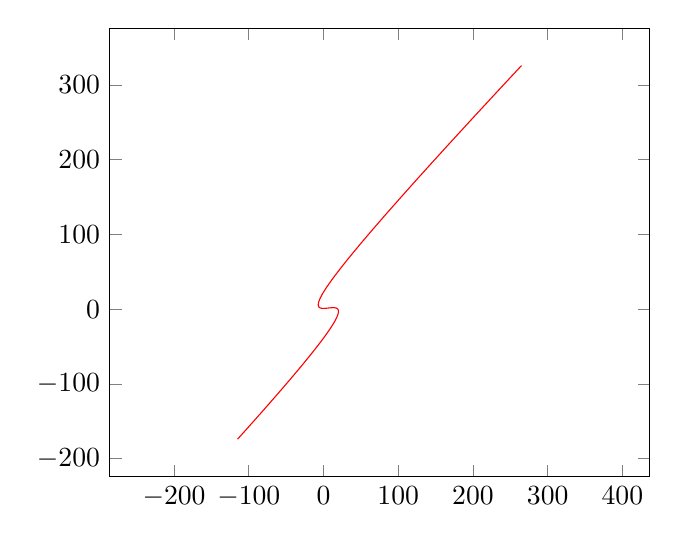
\begin{tikzpicture}
    \begin{axis}[
        trig format plots=rad,
        axis equal
    ]
    \addplot [samples=200, red]
      ({2*pow(x,3)+3*pow(x,2)-12*x}, {2*pow(x,3)+3*pow(x,2)+1});
    \end{axis}
  \end{tikzpicture}
\end{center}
\begin{align*}
  \frac{\diff{x}}{\diff{t}} &= 6t^{2}+6t-12 \\
  &= 6(t^{2}+t-2) \\
  \frac{\diff{y}}{\diff{t}} &= 6t^{2}+6t \\
  &= 6t(t+1) \\
  \frac{\diff{y}}{\diff{x}} &=
    \frac{\frac{\diff{y}}{\diff{t}}}{\frac{\diff{x}}{\diff{t}}} \\
  &= \frac{6t(t+1)}{t(t^{2}+t-2)} \\
  &= \frac{t(t+1)}{(t+2)(t-2)}
\end{align*}

\subsection*{Example 3}
Find the points at which the function is convex:
\[ x = \cos(2t) \quad y = \cos(t) \quad 0 < t < \pi \]
\begin{center}
  \begin{tikzpicture}
    \begin{axis}[
        trig format plots=rad,
        axis equal
    ]
    \addplot [samples=200, red]
      ({cos(2 * x)}, {sin(x)});
    \end{axis}
  \end{tikzpicture}
\end{center}
\begin{align*}
  \frac{\diff{x}}{\diff{t}} &= -2\sin(2t) \\
  \frac{\diff{y}}{\diff{t}} &= -\sin^{2}(t) \\
  \frac{\diff{y}}{\diff{x}} &=
    \frac{\frac{\diff{y}}{\diff{t}}}{\frac{\diff{x}}{\diff{t}}} \\
  &= \frac{-\sin(t)}{-2\sin(2t)} \\
  &= \frac{\sin(t)}{2\times2\sin(t)\cos(t)} \\
  &= \frac{\sec(t)}{4} \\
  \frac{\Diff{2}{y}}{\diff{x}^{2}} &=
    \frac{\frac{\diff}{\diff{t}}(\frac{\diff{y}}{\diff{x}})}
      {\frac{\diff{x}}{\diff{t}}} \\
  &= \frac{\sec(t)\tan(t)}{4}\times\frac{1}{-2\sin(2t)} \\
  &= -\frac{\sec(t)\tan(t)}{8\sin(2t)} \\
  &= -\frac{\sin(t)}{8\cos(t)\cos(t)2\sin(t)\cos(t)} \\
  &= -\frac{\sec^{3}(t)}{16}
\end{align*}
The function is convex wherever \( \frac{\Diff{2}{y}}{\diff{x}^{2}} > 0 \):
\[ -\frac{\sec^{3}(t)}{16} > 0 \]
\[ \sec^{3}(t) < 0 \]
\[ \sec(t) < 0 \]
\[ \cos(t) < 0 \]
\[ \frac{\pi}{2} < t < \frac{3\pi}{2} \]
Since we were given the precondition \( 0 < t < \pi \), we only care about the
interval:
\[ \frac{\pi}{2} < t < \pi \]

\subsection*{Example 4}
Find the equation of the tangent line at (4,3):
\[ x = 3t^{2}+1 \quad y = 2t^{3}+1 \]
\begin{center}
  \begin{tikzpicture}
    \begin{axis}[
        trig format plots=rad,
        axis equal
    ]
    \addplot [samples=200, red]
      ({3*pow(x,2)+1}, {2*pow(x,3)+1});
    \end{axis}
  \end{tikzpicture}
\end{center}
The equation of the tangent line is of the form:
\[ y-y_{1}=m(x-x_{1}) \mathrm{\ where\ } m = \frac{\diff{y}}{\diff{x}} \]
\begin{align*}
  \frac{\diff{x}}{\diff{t}} &= 6t \\
  \frac{\diff{y}}{\diff{t}} &= 6t^{2} \\
  \frac{\diff{y}}{\diff{x}} &=
    \frac{\frac{\diff{y}}{\diff{t}}}{\frac{\diff{x}}{\diff{t}}} \\
  &= \frac{6t^{2}}{6t} \\
  &= t
\end{align*}
Tangent line at (4,3):
\begin{align*}
  y-y_{1} &= \frac{\diff{y}}{\diff{x}}(x-x_{1}) \\
  y-y_{1} &= t(x-x_{1}) \\
  3-(2t^{3}+1) &= t(4-(3t^{2}+1)) \\
  3-2t^{3}-1 &= y(4-3t^{2}-1) \\
  2-2t^{3} &= 4t-3t^{3}-t \\
  t^{3}-3t+2 &= 0 \\
  t^{3}-t^{2}+t^{2}-t-2t+2 &= 0 \\
  t^{2}(t-1)+t(t-1)-2(t-1) &= 0 \\
  (t-1)(t^{2}+t-2) &= 0 \\
  (t-1)(t+2)(t-1) &= 0 \\
  (t-1)^{2}(t-2) &= 0
\end{align*}
\[ t = 1 \quad t = 2 \]
At \( t = 1 \), \( (x, y) = (4,3) \), therefore the equation of the tangent
line is:
\begin{align*}
  y-3 &= 1(x-4) \\
  y &= x - 1
\end{align*}

\subsection*{Example 5}
Find the arc length of the curve:
\[ x = \e^{t}+\e^{-t} \quad y = 5-2t \quad 0 \leq t \leq 3 \]
\begin{center}
  \begin{tikzpicture}
    \begin{axis}[
        trig format plots=rad,
        axis equal
    ]
    \addplot [samples=200, red]
      ({pow(e, x)+pow(e, -x)}, {5-2*x});
    \end{axis}
  \end{tikzpicture}
\end{center}
\begin{align*}
  L &= \int_{a}^{b}{\sqrt{1+(f'(x))^{2}}\diff{x}} \\
  f'(x) &= \frac{\diff{y}}{\diff{x}} =
    \frac{\diff{y}/\diff{t}}{\diff{x}/\diff{t}} \\
  L &= \int_{a}^{b}{\sqrt{(\frac{\diff{x}}{\diff{t}})^{2}+
      (\frac{\diff{y}}{\diff{t}})^{2}}\diff{t}} \\
  &= \int_{0}^{3}{\sqrt{(\e^{t}-\e_{-t})^{2}+(-2)^{2}}\diff{t}} \\
  &= \int_{0}^{3}{\sqrt{\e^{2t}+\e^{-2t}-2\e^{t}\e^{-t}+4}\diff{t}} \\
  &= \int_{0}^{3}{\sqrt{\e^{2t}+\e^{-2t}+2}} \\
  &= \int_{0}^{3}{\sqrt{(\e^{t}+\e^{-t})^{2}}\diff{t}} \\
  &= \int_{0}^{3}{(\e^{t}+\e^{-t})\diff{t}} \\
  &= \bigg[\e^{t}-\e^{-t}\bigg]_{0}^{3} \\
  &= \e^{3}-\e^{-3}
\end{align*}

\subsection*{Example 6}
Find the surface area of the solid of revolution:
\[ x = 3t-t^{2} \quad y = 3t^{2} \quad 0 \leq t \leq 1 \]
\begin{center}
  \begin{tikzpicture}
    \begin{axis}[
        trig format plots=rad,
        axis equal
    ]
    \addplot [samples=200, red]
      ({3*x-pow(x,2)}, {3*pow(x,2)});
    \end{axis}
  \end{tikzpicture}
\end{center}
\begin{align*}
  S &= \int{2\pi y\diff{S}} \\
  &= \int_{a}^{b}{2\pi y\sqrt{1+(\frac{\diff{y}}{\diff{x}})^{2}}\diff{x}} \\
  &= 2\pi\int_{a}^{b}{y\sqrt{(\frac{\diff{x}}{\diff{t}})^{2}+
    (\frac{\diff{y}}{\diff{t}})^{2}}\diff{t}} \\
  &= 2\pi\int_{0}^{1}{(3t^{2})\sqrt{(3-2t^{2})^{2}+(6t)^{2}}\diff{t}} \\
  &= 6\pi\int_{0}^{1}{t^{2}\sqrt{9+9t^{4}-12t^{2}+36t^{2}}\diff{t}} \\
  &= 6\pi\int_{0}^{1}{t^{2}\sqrt{3^{2}+(3t^{2})^{2}+2(3)(3t^{2})}\diff{t}} \\
  &= 6\pi\int_{0}^{1}{t^{2}\sqrt{(3+3t^{2})^{2}}\diff{t}} \\
  &= 6\pi\int_{0}^{1}{t^{2}(3+3t^{2})\diff{t}} \\
  &= 18\pi\int_{0}^{1}{(t^{2}+t^{4})\diff{t}} \\
  &= 18\pi\bigg[\frac{t^{3}}{3}+\frac{t^{5}}{5}\bigg]_{0}^{1} \\
  &= 18\pi(\frac{1}{3}+\frac{1}{5}) \\
  &= 18\pi(\frac{8}{15}) \\
  &= \frac{48\pi}{5}
\end{align*}

\subsection*{Example 7}
\[ x = a\cos(\theta) \quad y = b\sin(\theta) \quad 0 \leq \theta \leq 2\pi \]
\[ \cos(\theta) = \frac{x}{a} \]
\[ \sin(\theta) = \frac{y}{b} \]
\[ \sin^{2}(\theta)+\cos^{2}(\theta) =
   \frac{x^{2}}{a^{2}}+\frac{y^{2}}{b^{2}} = 1 \]
\begin{center}
  \begin{tikzpicture}
    \begin{axis}[
        trig format plots=rad,
        axis equal
    ]
    \addplot [samples=200, red]
      ({1*cos(x)}, {3*sin(x)});
    \end{axis}
  \end{tikzpicture}
\end{center}
\begin{align*}
  A &= 4\int_{a}^{b}{y\diff{x}} \\
  &= 4\int_{\pi/2}^{0}{(b\sin(\theta))(-a\sin(\theta))\diff{\theta}} \\
  &= -4ab\int_{\pi/2}^{0}{\sin^{2}(\theta)\diff{\theta}} \\
  &= 4ab\int_{0}^{\pi/2}{\frac{1}{2}-\frac{1}{2}\cos(2\theta)\diff{theta}} \\
  &= 2ab\int_{0}^{\pi/2}{1-\cos(2\theta)\diff{\theta}} \\
  &= 2ab\bigg[\theta-\frac{\sin(2\theta)}{2}\bigg]_{0}^{\pi/2} \\
  &= 2ab\bigg[(\frac{\pi}{2}-\frac{\sin(\pi)}{2})-
    (0-\frac{\sin(\theta)}{2})\bigg] \\
  &= ab\pi
\end{align*}

\subsection*{Problem 33}
Find the area under the curve bounded by:
\[ x = 1+\e^{t} \quad y = t-t^{2} \]
and the x-axis:
\begin{center}
  \begin{tikzpicture}
    \begin{axis}[
        trig format plots=rad,
        axis equal
    ]
    \addplot [samples=200, red]
      ({1+pow(e, x)}, {x-x^2});
    \end{axis}
  \end{tikzpicture}
\end{center}
\[ A = \int_{a}^{b}{y\diff{x}} \]
\[ y = 0 = t-t^{2} \]
\[ t(1-t) = 0 \]
\[ t = 0 \quad (x = 2) \quad \quad t = 1 \quad (x=1+\e) \]
\begin{align*}
  A &= \int_{2}^{1+\e}{y\diff{x}} \\
  &= \int_{x=2}^{x=1+\e}{(t-t^{2})\diff{x}} \\
  &= \int_{0}^{1}{(t-t^{2})\e^{t}\diff{t}} \\
  &= (t-t^{2})\e^{t}-\int{(1-2t)\e^{t}\diff{t}}
    \quad\mathrm{(Integration\ By\ Parts)} \\
  &= t(1-t)\e^{t}-\bigg[(1-2t)\e^{t}-\int{-2\e^{t}\diff{t}}\bigg] \\
  \int_{0}^{1}{(t-t^{2})\e^{t}\diff{t}} &=
    \bigg[t(1-t)\e^{t}-(1-2t)\e^{t}-2\e^{t}\bigg]_{0}^{1} \\
  &= 3-\e
\end{align*}

\begin{center}
  You can find all my notes at \url{http://omgimanerd.tech/notes}. If you have
  any questions, comments, or concerns, please contact me at
  alvin@omgimanerd.tech
\end{center}

\end{document}
